
\section{Mô hình sinh cử chỉ}

%\begin{frame}{Tổng quan về bài toán}
%%	\begin{figure}
%%		\centering
%%		\includegraphics[width=0.8\linewidth]{SequenceGesture.jpg}
%%	\end{figure}
%%	
%	Cho chuỗi cử chỉ $\mathbf{g} \in \mathbb{R}^{(N+ M) \times D}$, với $\mathbf{s} \in \mathbb{R}^{N \times D}$ và đoạn cử chỉ nhãn $\mathbf{x}_0 \in \mathbb{R}^{M \times D}$ với $D=1141$, $N=8$, $M=80$. Chuỗi âm thanh $\mathbf{a} \in \mathbb{R}^{64000}$ (4s: $16000$ sample rate). Cảm xúc $\mathbf{e} \in \mathbb{R}^6$. 
%%	$\{\beta_t \in (0, 1)\}_{t=1}^T$
%
%\end{frame}


\begin{frame}{Diffusion cho bài toán sinh cử chỉ}
	\textbf{Điểm giống}
	\begin{itemize}
		\item Sử dụng mô hình Diffusion \cite{yang2023diffusestylegesture} trên cử chỉ $\bx^{1:M \times D}$,  với $M$ frame theo thời gian, $D=1141$ là các điểm toạ độ chuyển động của mỗi khung hình (tương tự width và height trong ảnh).
		\item Classifier-Free Diffusion Guidance với $\bx_0$ objective.
		\item Latent vector có số chiều là $256$.
		\end{itemize}
		
		\textbf{Điểm khác}
		
		\begin{itemize}
			\item Sinh cử chỉ có điều kiện:
			\begin{itemize}
				\item Điều kiện cảm xúc: $c = \big[ \mathbf{s}, \mathbf{e}, \mathbf{a} \big]$ và $c_{\varnothing} = \big[ \varnothing, \varnothing, \mathbf{a} \big]$.
				\item Nội suy trạng thái giữa hai cảm xúc $\mathbf{e}_1, \mathbf{e}_2$, sử dụng điều kiện: $c = \big[ \mathbf{s}, \mathbf{e}_1, \mathbf{a} \big]$ và $c_{\varnothing} = \big[ \mathbf{s}, \mathbf{e}_2, \mathbf{a} \big]$.
			\end{itemize}
			\item Self-Attention: Mối liên hệ giữa các cảm xúc, cử chỉ khởi tạo và từng frame (tương tự DALL-E 2 - mối liên hệ giữa văn bản và ảnh).
			\item Concat âm thanh (Giống ControlNet - Pixel-wise Condition)
%			\item Học mối liên hệ giữa điều kiện và các frame bằng Local-Cross Attention
		\end{itemize}
\end{frame}

\begin{frame}{Tổng quan các công đoạn}
	
	\begin{figure}
		\centering
		\includegraphics[width=\linewidth]{AllStage}
	\end{figure}
	
\end{frame}

\begin{frame}{Các công đoạn trong mô hình OHGesture}
	\begin{figure}
		\centering
		\includegraphics[width=\linewidth]{ModelStage}
	\end{figure}
\end{frame}

\begin{frame}{Diffusion cho bài toán sinh cử chỉ}
	
	\begin{figure}
		\centering
		\includegraphics[width=0.9\linewidth]{OverviewArchitecture.jpg}
	\end{figure}
	
\end{frame}

\begin{frame}{Kiến trúc OHGesture}
	\begin{figure}
		\centering
		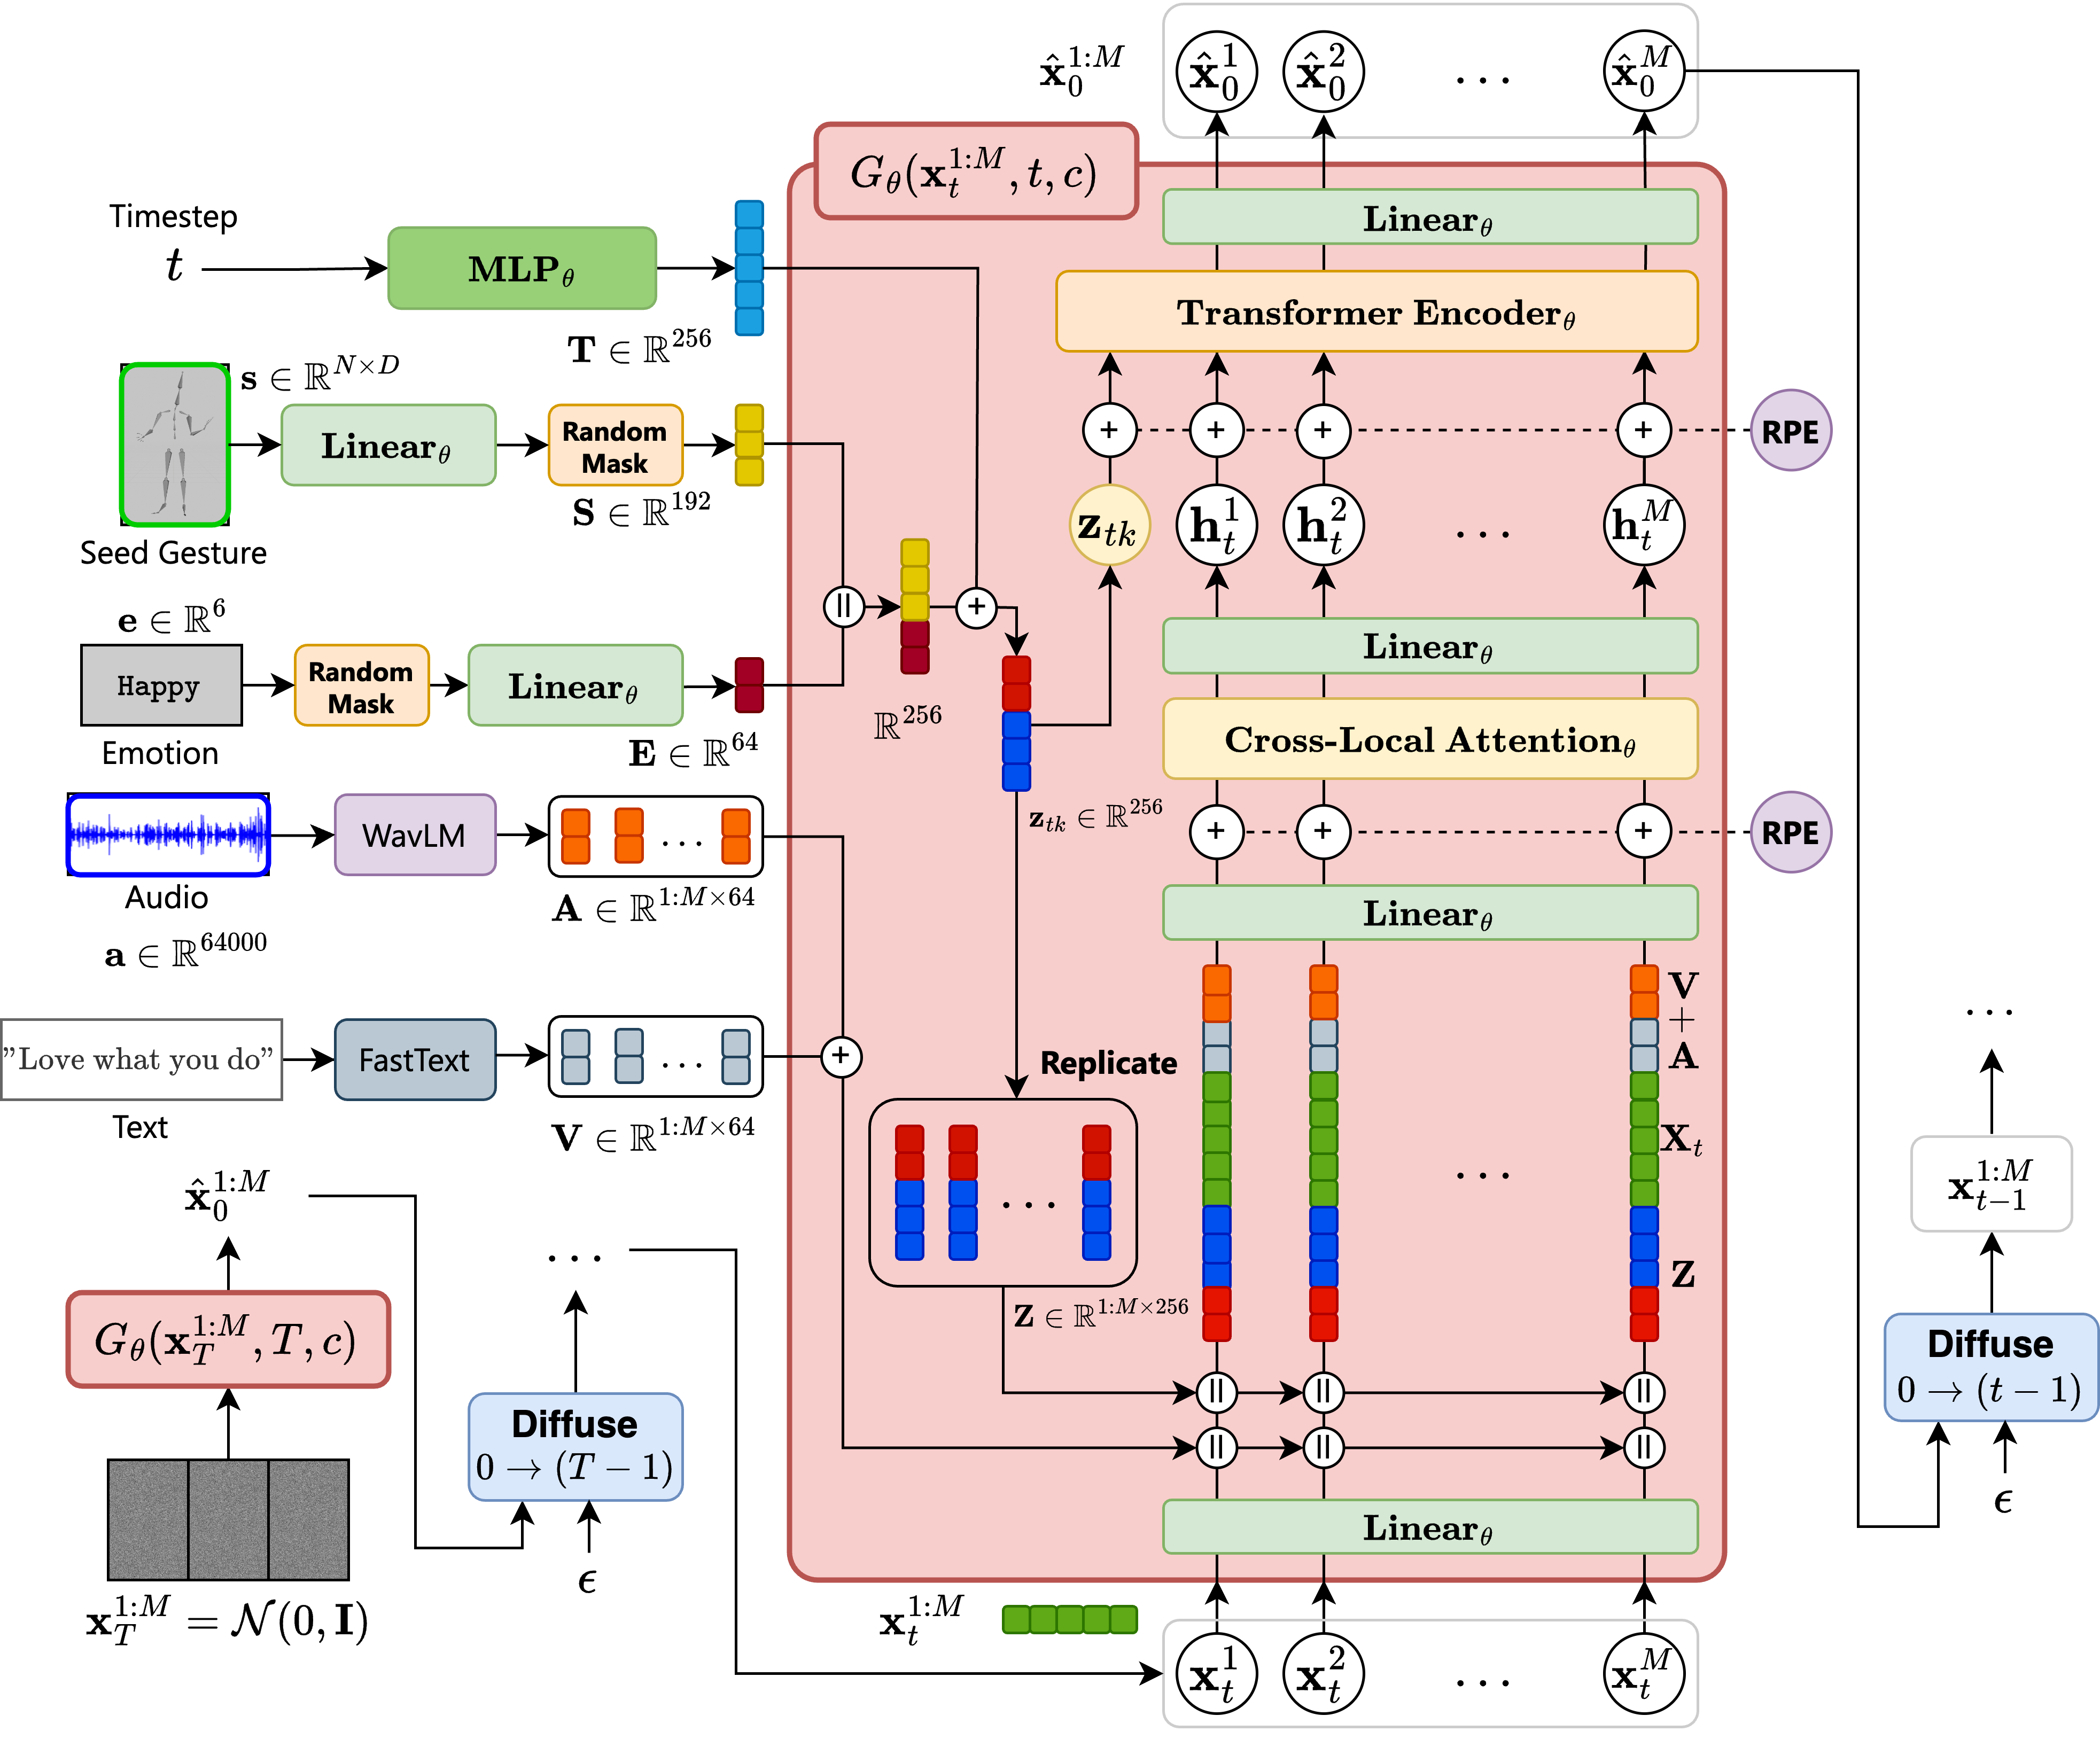
\includegraphics[width=0.9\linewidth]{OHGesture}
	\end{figure}
\end{frame}


\begin{frame}{Attention}
	\begin{figure}
		\centering
		\includegraphics[width=0.85\linewidth]{Attention}
	\end{figure}
\end{frame}

\begin{frame}{Cross-Local Attention and Self-Attention}
	\small
	\textbf{Cross-Local Attention}
	\begin{equation*} \label{eq:attention}
		\operatorname{Attention}(\mathbf{Q}, \mathbf{K}, \mathbf{V}, \mathbf{M})=\operatorname{softmax}\left(\frac{\mathbf{Q} \mathbf{K}^{T}+\mathbf{M}}{\sqrt{C}}\right) \mathbf{V}
	\end{equation*}
	

	\begin{columns}
%		Transfomer Encoder : 
		
		\begin{column}{0.5\textwidth}
				\textbf{Self-Attention}
			$$
			f_{\text{MultiHead}(\mathbf{X})} = \operatorname{concat} \left( \mathbf{H}_1, \mathbf{H}_2, \dots, \mathbf{H}_h \right) \mathbf{W}_O
			$$
			
			$$
			\mathbf{H}_i = \operatorname{softmax} \left( \frac{\mathbf{Q}_i \mathbf{K}_i^T}{\sqrt{d_k}} \right) \mathbf{V}_i
			$$
		\end{column}
		
		\begin{column}{0.5\textwidth}
			\begin{figure}
				\centering
				\includegraphics[width=\linewidth]{CrossLocalAttention}
			\end{figure}
		\end{column}
	\end{columns}

\end{frame}


%\begin{frame}
%	\begin{figure}
%		\centering
%		\includegraphics[width=0.8\linewidth]{DiffusionProcess}
%	\end{figure}
%\end{frame}


%\begin{figure} 
%	\centering
%	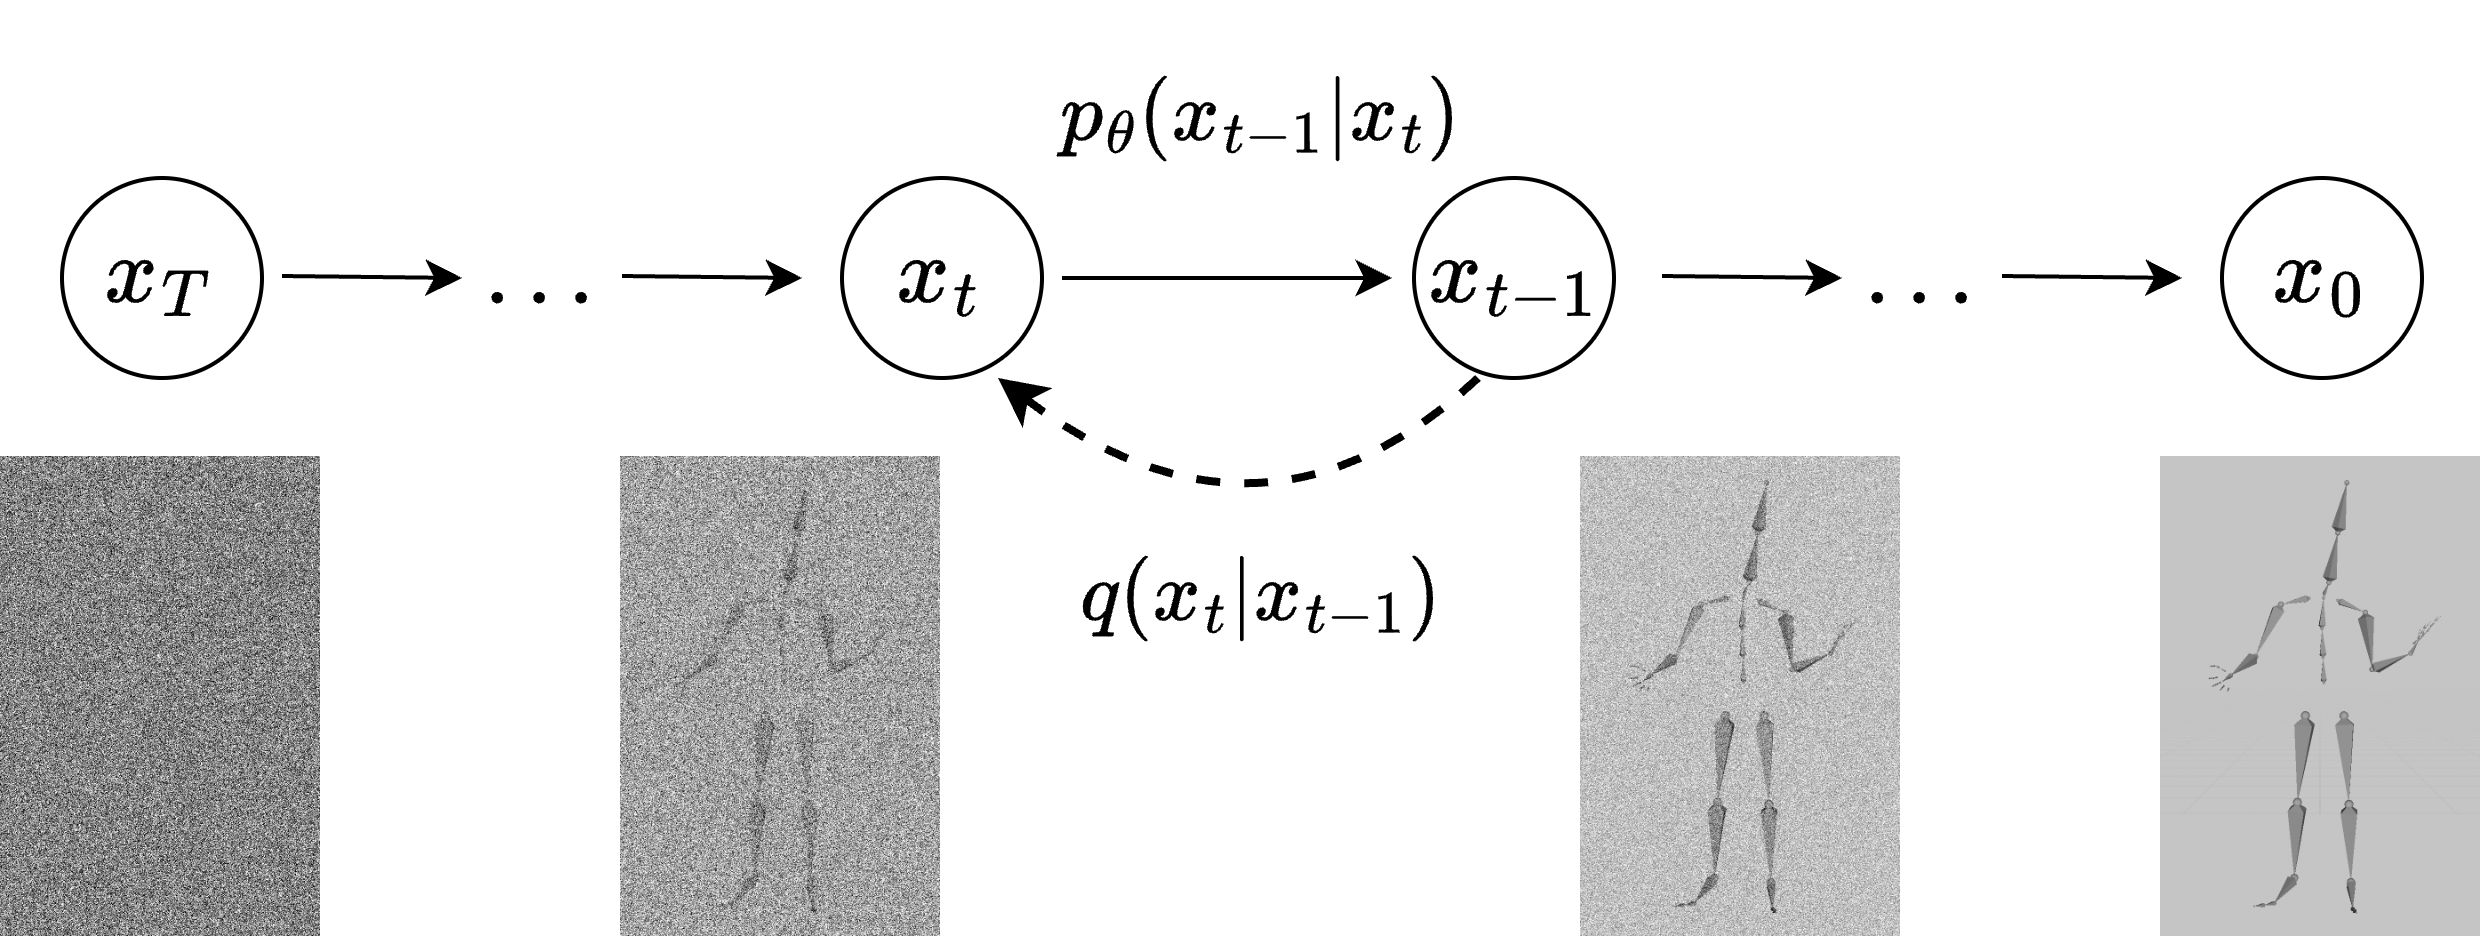
\includegraphics[width=0.8\linewidth]{DiffusionForward}
%\end{figure}


%\begin{frame}
%	
%	$
%	\label{Gaussian}
%	q\left(x_t \mid x_{t-1}\right)=\mathcal{N}\left(x_t ; \sqrt{1-\beta_t} x_{t-1}, \beta_t \mathbf{I}\right)
%	$
%	
%	$
%	\label{eq1}
%	q\left({x}_{1:T} \mid {x}_0\right)=\prod_{t=1}^T q\left({x}_t \mid {x}_{t-1}\right)
%	$
%	$
%	p_\theta\left({x}_{t-1} \mid {x}_t\right)=\mathcal{N}\left({x}_{t-1} ; {\mu}_\theta\left({x}_t, t\right), {\Sigma}_\theta\left({x}_t, t\right)\right)
%	$
%	
%	$
%	q\left({x}_t \mid {x}_0\right)=\mathcal{N}\left({x}_t ; \sqrt{\bar{\alpha}_t} {x}_0,\left(1-\bar{\alpha}_t\right) \mathbf{I}\right)
%	$
%	
%	$
%	\hat{x}_0=G\left(x_t, t, c\right)
%	$
%\end{frame}

	
%	\begin{columns}
	%		\begin{column}{0.5\textwidth}
		%			\textbf{DDPM (stochastic sampling):}
		%			\begin{itemize}
			%			\item Predict $x_0$ from $x_t$
			%			
			%			\item Convert to $\epsilon_{pred}$
			%			
			%			\item Use the formula:
			%			
			%			$$x_{t-1} = \frac{1}{\sqrt{\alpha_t}} x_t - \frac{1-\alpha_t}{\sqrt{1-\bar{\alpha}t}\sqrt{\alpha_t}} \epsilon_{\text{pred}} + \sigma_t z$$
			%			
			%			\item where $z \sim \mathcal{N}(0,I)$ is random noise
			%			\end{itemize}
		%			
		%		\end{column}
	%		
	%		\begin{column}{0.5\textwidth}
		%			\textbf{DDIM (deterministic sampling):}
		%			
		%			Predict $x_0$ from $x_t$
		%			
		%			NO additional noise term ($\sigma_t = 0$)
		%			
		%			Use the formula:
		%			
		%			$x_{t-1} = \sqrt{\bar{\alpha}{t-1}} x_0^{\text{pred}} + \sqrt{1-\bar{\alpha}_{t-1}} \epsilon_{\text{pred}}$
		%			
		%			Where:
		%			\begin{itemize}
			%			\item $\bar{\alpha}_t$ is the cumulative product of $\alpha$'s from 1 to t
			%			\item $\epsilon_{pred}$ is derived from $x_0$ prediction using:
			%			\item $\epsilon_{pred} = \frac{x_t - \sqrt{\alpha_t}x_{0_{pred}}}{\sqrt{1-\alpha_t}}$
			%			\end{itemize}
		%		\end{column}
	%	\end{columns}
	
